\documentclass{article}
\usepackage{graphicx}
\usepackage{hyperref}
\graphicspath{{images/}}

\begin{document}

\title{Parallelizing Convex Learning Algorithms}
\author{Michael Curtis 260475694\\
Voula Theophanous 260480568}
\maketitle

\begin{abstract}

This report outlines methodologies for parallalizing convex cost function machine learning algorithms. We present a Master-Worker implementation and a Gradient-Gossip based implementation. Both of these methods aim to minimize the amount of communications between processes and maximize the amount of parallel execution. We will also describe what a convex function is, how convexity relates to learning algorithms, and why convex learning algorithms can be easily parallized.

\end{abstract}

\section{Introduction}
The following example illustrates why executing a machine algorithms faster could be important. Imagine you are a computer scientist for the World Health Organization. There has been an outbreak of a mosquito born virus that has been growing in western Aftrican countries. It has been found that spraying airborne pesticides to control misquito population is effective in controlling the spread of the virus. Your organization has 140 teams deligated to spraying the pesticides across the effected countries. You have over 3000 mosquito hotspots near population centers where mosquitos' blood have been testing at high rates for the virus. You are given the location of mosquito blood testing, associated rate of virus accurance in mosquito and population centers, and previous pesticide sprays with associated location. You have decided to build a linear regression model aiming to minimize the total number of mosquito positive virus tests. Since there are hundreds or thousands of features in our training data the model takes days to build when running in serial. If we have a method to parallelize this learning algorithm we could send the 140 teams to an optimally choosen 140 of the 3000 locations in the magnitude of hours.

\subsection{Definition: Convex Functions}
The simple and informal definition of a convex function is to visualize a parabola, where we can easily see that there is only one global minimum. That is there is only one set of parameters to the derivative of the function that will return 0. Lets try to visualize this in general. Pick two sets of parameters to the function that given us two different points on the functions. With the two points draw a line connecting, or in the higher dimensional case, visualize a surface where both the points are contained. If for any two points of any parameters has an obstruction disallowing a line of sight from one point to another, the function is not convex as there will be multiple parameter values such that the derivative of the function evaluates to 0. This is mathematically defined in Stanford Professor Stephen Boyd's textbook\footnote{\url{https://web.stanford.edu/~boyd/cvxbook/bv_cvxbook.pdf}} \\
\\
A function $f:R^n \rightarrow R$ is \textit{convex} if $domain f$ is a convex set and if for all $x,y \in domain f$, and $\theta$ with $0 \leq \theta \leq 1$, we have
\begin{equation}
    \label{simple_equation}
    f(\theta x + (1 - \theta)y) \leq \theta f(x) + (1 - \theta)f(y)
\end{equation}
\begin{figure}[h]
    \centering
    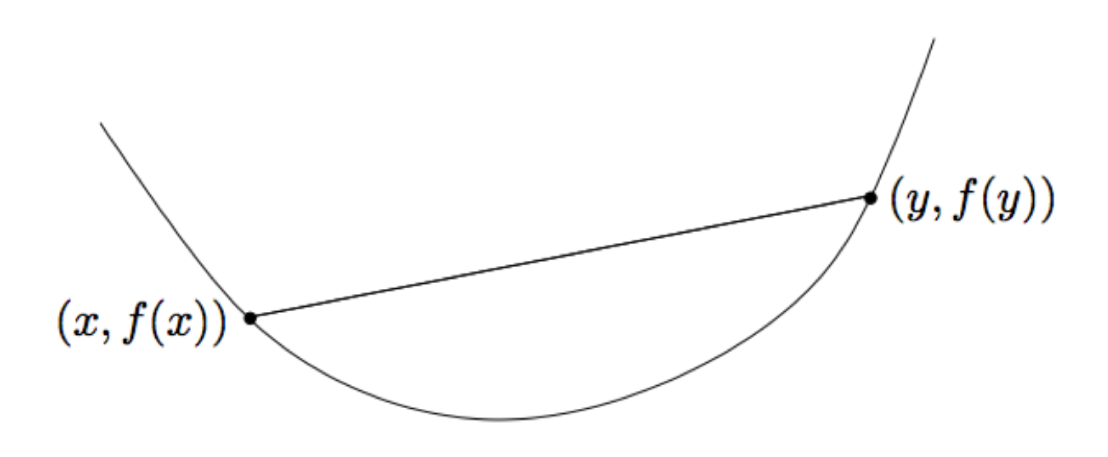
\includegraphics[width=3.0in]{convexboyd}
    \caption{A "chord" Between Two Points In a Convex Function}
    \label{convexboyd}
\end{figure}

\subsection{Convexity and Machine Learning}
Many machine learning algorithms boil down to solving a convex optimization problem. When we look for 
\\


\section{Conclusion}
Write your conclusion here.

\end{document}
